\documentclass[11pt]{article}
% Language setting
% Replace `english' with e.g. `spanish' to change the document language
\usepackage[english]{babel}

% Set page size and margins
% Replace `letterpaper' with `a4paper' for UK/EU standard size
\usepackage[letterpaper,margin=1in]{geometry}
% Useful packages
\usepackage{amsmath, amssymb, amsthm}
\usepackage{graphicx}
\usepackage[colorlinks=true, allcolors=blue]{hyperref}
\usepackage{algorithm}
\usepackage{algpseudocode}

\newtheorem{theorem}{Theorem}
\newtheorem{lemma}{Lemma}
\newtheorem{definition}{Definition}
\newcommand{\example}{\noindent\textbf{Example.\  }}
\newcommand{\exercise}{\noindent\textit{Exercise.\  }}
\newcommand{\remark}{\noindent\textit{Remark.}}


\renewcommand{\P}{\mathbb{P}}
\newcommand{\E}{\mathbb{E}}
\newcommand{\var}{\text{var}}
\newcommand{\mc}[1]{\mathcal{#1}}
\newcommand{\cE}{\mathcal{E}}
\newcommand{\1}[1]{\mathbf{1}\left\{#1\right\}}

\usepackage{pgfplots}
\usepgfplotslibrary{fillbetween}
\pgfmathdeclarefunction{gauss}{2}{\pgfmathparse{1/(#2*sqrt(2*pi))*exp(-((x-#1)^2)/(2*#2^2))}}


\title{MKTG 596: Adaptive Experimental Design Methods}
\author{Lalit Jain}

\begin{document}
\maketitle

\section{Introduction}

This course is about the algorithms and techniques that drive experimentation in online platforms. At many firms, thousands of experiments are run daily to gather the vast amount of data needed to enable data-driven decision-making. For any one of these experiments, an experimenter faces the challenge of deciding what data to collect, how long to run the experiment, and how to glean insights from the data collected. As a result, there is an increased demand by practitioners for methods and algorithms that deliver statistically sound results faster and with less opportunity cost. This course develops a modern toolbox of experimentation, with a focus on adaptive experimental design. Rooted in classical statistical and machine learning techniques, AED decides what future data to collect based on past measurements in a closed loop. Due to both theoretical gains and empirical success, AED has quickly become one of the most commonly employed algorithmic paradigms in practice with a promise of cutting experimentation time by up to half. However, practitioners who employ AED blindly can easily bias their results, or potentially not collect the data needed to make any useful inferences.  

In practice experimental systems need to 
\begin{itemize}
    \item Return results rapidly (minimize sample complexity)
    \item Reduce opportunity cost (minimize regret)
    \item Provide valid inference (valid confidence intervals)
    \item Be robust to time variation
    \item Effectively incorporate customer heterogeneity
\end{itemize}
In addition, 
As we will see in this course, unfortunately there is no master algorithm and practitioners often have to trade-off several competing objectives. 

The course is organized as follows:
\begin{itemize}
    \item We begin with a short overview and discussion of the three pillars of experimentation, A/B Testing, Multi-Armed Bandits, and Multiple Hypothesis Testing
    \item Building upon our experience with SPRT and MAB we will next discuss Anytime-Valid-Inference
    \item This will be followed by a more in-depth discussion of MAB with a focus on Optimistic Strategies, such as MAB and Thompson Sampling. 
    \item Contextual Bandits
    \item Interference in Experiments
    \item Off Policy Evaluation
    \item Experimental Design
    \item Orthogonal ML
    \item Reinforcement Learning
\end{itemize}

\section{Three Pillars}

\subsection{Pillar 1: A/B Testing}
The following captures a common setting in online A/B testing and statistics.

\example We have a single distribution that is assumed to be Gaussian $N(\mu,1)$, and we have collected samples $X_1, \cdots, X_n$ from this distribution. 

\begin{tikzpicture}
\begin{axis}[
    axis lines=left,
    enlargelimits=upper,
    xlabel=$x$,
    ylabel=$y$,
    no markers,
    smooth,
    ticks=none,
]

% Gaussian parameters
\def\mu{1}
\def\delta{2}
\def\tau{2.2}
\def\sigma{1}

% Gaussian distributions
\addplot[name path=gauss1, thick, domain=-3+\mu:3+\mu, samples=100] {gauss(\mu, \sigma)};
\addplot[name path=gauss2, thick, domain=-3+\mu+\delta:3+\mu+\delta, samples=100] {gauss(\mu+\delta, \sigma)};

% Vertical line at tau
\addplot[name path=tau, domain=0:0.5] coordinates {(\tau, 0)(\tau, 0.5)};

% Fill areas
\path[name path=axis] (axis cs:\tau,0) -- (axis cs:\tau,0.5);
\addplot[fill=red!20, opacity=0.5] fill between[of=gauss1 and axis, soft clip={domain=\tau:3+\mu}];
\addplot[fill=blue!20, opacity=0.5] fill between[of=gauss2 and axis, soft clip={domain=-3+\mu+\delta:\tau}];

% Labels
\node at (axis cs:\mu, -0.05) [below] {$\mu$};
\node at (axis cs:\mu+\delta, -0.05) [below] {$\mu + \Delta$};
\node at (axis cs:\tau, -0.05) [below] {$\tau$};
%\node[red] at (axis cs:\mu, 0.4) {$f_1(x)$};
%\node[blue] at (axis cs:\mu+\delta, 0.4) {$f_2(x)$};


\end{axis}
\end{tikzpicture}

Consider the following hypothesis test:
\begin{align*}
    H_ 0&: \mu = \mu_0\\
    H_1&: \mu = \mu_0 +\Delta
\end{align*}
where $\mu_0$ and $\Delta$ are known. In practice, $\mu_0$ could be known because the control variant may have been running for many months. The ``gap'' $\Delta$ is known as the \textit{minimum detectable effect} and captures the smallest deviation from the control that we are interested in capturing.

We consider the following test. Choose a threshold $\tau$, if $\bar{x} = \frac{1}{n}\sum_{i=1}^n X_i > \tau$ then we will declare for $H_1$ otherwise we declare for $H_0$. We want this test to have a type-1 error bounded by $\alpha$, and a type-2 error bounded by $\beta$. That is, the probability we accept the alternative given that the null is true is at most $\alpha$, and the probability we accept the null given the alternative is at most $\beta$.

A natural question is how to choose $\tau, n$ to guarantee this result. This is a common problem considered in most introductory statistics courses, and we quickly review it. Define $z_{\alpha} = \Phi^{-1}(1-\alpha)$. To guarantee that the type-1 error is indeed bounded by $\alpha$ we need
\begin{align*}
    \frac{\tau - \mu_0}{\sqrt{1/n}} \geq z_{\alpha} 
\end{align*}
where $\Phi$ is the CDF function for a $N(0,1)$. Similarly for the type-2 error,
\begin{align*}
    \frac{\tau - (\mu_0+\Delta) }{\sqrt{1/n}} \leq -z_{\beta} 
\end{align*}
See Figure~\ref{}.

Adding these together, we see that it suffices to take
\begin{align*}
    n \geq \frac{(z_{\alpha} + z_{\beta})^2}{\Delta^2}
\end{align*}

Now consider the specific case where $\beta = \alpha = \delta$. Using the fact that $1-\Phi(t) \leq e^{-t^2/2}$ and that $\Phi(t)$ is monotonically increasing, we can upper bound $z_{\delta}\leq \sqrt{2\log(1/\delta)}$, so we see that with probability greater than $1-2\delta$, if $n\geq 8\log(1/\delta)/\Delta^2$ we will return the correct hypothesis. \qed\\


\noindent\textbf{Lower Bounds. } The natural question to ask is, how tight is this? Can we do better? In fact, we can prove a lower bound. Recall that the KL-Divergence between two distributions $p_0, p_1$ (supported on $\mathbb{R}$) is 
\begin{equation*}
    KL(p_0, p_1) = \int \log\left(\frac{p_0(x)}{p_1(x)}\right) p_0(x) dx
\end{equation*}

\begin{theorem}
Any hypothesis test $\Psi$ that can distinguish $H_0: X_1,\cdots, X_n \sim p_0$ and $H_1: X_1,\cdots, X_n \sim p_1$ has a probability of error lower bounded by 
\[\max(\P_0(\Psi=1), \P_1(\psi=0))\geq \frac{1}{4}e^{-nKL(p_0, p_1)}\]
\end{theorem}
\begin{proof}
Without loss of generality, we refer to the 

\begin{align*}
\max(\P_0(\Psi=1), \P_1(\psi=0))
&\geq \frac{1}{2}\left(\P_0(\Psi=1) + \P_1(\psi=0))\right)\\
&= \frac{1}{2}\left(\int_{\psi=1} dp_0  + \int_{\psi=0} dp_1\right)\\
&\geq \frac{1}{2}\int \min(dP_0, dP_1)
\end{align*}

Now note that a) $\int \max(dp_0, dp_1) \leq 2$ (since the max is less than the sum), and b) \[\int \min(dp_0, dp_1)\int \max(dp_0, dp_1)\geq (\int \sqrt{ \min(dp_0, dp_1) \max(dp_0, dp_1)})^2\]. Thus
\begin{align*}
    \max(\P_0(\Psi=1), \P_1(\psi=0)) 
    &\geq \frac{1}{4} (\int \sqrt{dp_0 dp_1})^2\\
    &= \frac{1}{4} (\int dp_0\sqrt{ \frac{dp_1}{dp_0}})^2\\
    &= \frac{1}{4} \exp[2\log\left(\int dp_0\sqrt{ \frac{dp_1}{dp_0}}\right)]\\
    &\geq \frac{1}{4} \exp[2\int\log(\sqrt{ \frac{dp_1}{dp_0}})dp_0] \tag{Jensen's inequality}\\
    &= \frac{1}{4} \exp[-\int\log(\sqrt{ \frac{dp_0}{dp_1}})dp_0]\\
    &= \frac{1}{4} \exp[-\int\log(\frac{dp_0}{dp_1})dp_0]\\
    &= \frac{1}{4} \exp(-KL(p^n_0, p^n_1))
\end{align*}
\textit{Exercise:} Show that $KL(p^n_0, p^n_1) = nKL(p_0, p_1)$
\end{proof}

For our setting above, $KL(N(\mu, 1), N(\mu+\Delta,1)) = \Delta^2/2$ so we see that 
\[\max(\P_0(\Psi=1), \P_1(\psi=0)) \geq \frac{1}{4} \exp(-n\Delta^2/2)\]
Thus, our probability of error will be at least $\delta$ unless $n \geq 2\log(1/\delta)/\Delta^2$. You will notice that this is a factor of 4 tighter than our upper bound. How can we do better? Answer: Adaptive Experimentation, namely the Sequential Probability Ratio Test. 


\subsection{The Sequential Probability Ratio Test}
Let's return to our hypothesis testing setting. 
\begin{align*}
    H_0&: X_1,\cdots, X_n \sim p_0\\
    H_1&: X_1,\cdots, X_n \sim p_1
\end{align*}

Indeed, denote the expectation and probability measure with respect to $p_i, i=0,1$ as $\E_i$.

Define the \textit{likelihood ratio} $\Lambda_t = \prod_{s=1}^t \frac{p_1(X_s)}{p_0(X_s)}$, $t\leq n$. The SPRT choose two thresholds, $\gamma_0, \gamma_1$ with $\gamma_1 > \gamma_0$. The SPRT stops at a time $\tau$, and outputs $H_1$ if $\Lambda_{\tau} > \gamma_1$ and otherwise outputs $H_0$. Our goal is to set the thresholds to guarantee that Type-1,2 error are bounded by $\alpha, \beta$ respectively.  


To make the following argument precise, we will need to employ the fact that $\Lambda_t$ forms a Martingale sequence under $\mathbb{P_0}$.  Then 
\begin{align*}
    \E[\Lambda_t|X_1, \cdots, X_{t-1}] = \Lambda_{t-1} \E_0\left[\frac{p_1(X_{t})}{p_0(X_{t})}\right] = \Lambda_{t-1} 
\end{align*}
Similarly, $\Lambda_t^{-1}$ forms a martingale sequence under $P_1$.



\newcommand{\lambdatau}{\Lambda_{\tau}}
Let $x = (X_1, \cdots, X_n)$, and abusing notation, we let $p_0(x) = p(X_1)\cdots p(X_n)$. Again letting $\alpha$ denote our Type 1 error and $\beta$ to denote our Type 2 error, we compute:
we now compute 
\begin{align*}
    1-\beta 
    &= \P_1(\lambdatau > \gamma_1) \\
    &= \int_{\Lambda_{\tau} > \gamma_1} p_1(x) dx\\
    &= \int_{\Lambda_{\tau} > \gamma_1} \frac{p_1(x)}{p_0(x)} p_0(x)dx\tag{Wald's Ratio Identity}\\
    &\geq \gamma_1 \int_{\Lambda_{\tau} > \gamma_1} p_0(x) dx \\
    &= \gamma_1\alpha
\end{align*}
% and similarly 
% \begin{align*}
%     \beta 
%     &= \P_1(\lambdatau < \gamma_0) \\
%     &= \int_{\Lambda_{\tau} < \gamma_0} p_1(x) dx\\
%     &= \int_{\Lambda_{\tau} < \gamma_0} \frac{p_1(x)}{p_0(x)} p_0(x)dx\tag{Wald's Ratio Identity}\\
%     &\leq \gamma_0 \int_{\Lambda_{\tau} < \gamma_0} p_0(x) dx \\
%     &\leq \gamma_0(1-\alpha)
% \end{align*}
and similarly 
\begin{align*}
    1-\alpha
    &= 1-\P_0(\lambdatau > \gamma_1) \\
    &= \int_{\lambdatau < \gamma_0} p_0(x) dx\\
    &= \int_{\lambdatau < \gamma_0} \frac{p_0(x)}{p_1(x)} p_1(x)dx\tag{Wald's Ratio Identity}\\
    &\geq \gamma_0^{-1} \int_{\Lambda_{\tau} < \gamma_0} p_1(x) dx \\
    &\geq \gamma_0^{-1}\beta
\end{align*}

The first series of inequalities implies that we should choose
\[\gamma_1 \leq \frac{1-\beta}{\alpha}\]
and similarly
\[\gamma_0 \geq \frac{\beta}{1-\alpha}\]
In general we set $\gamma_, \gamma_1$ to be equal to these values. 

This calculation demonstrates the trade-off between $\gamma_0, \gamma_1, \alpha, \beta$. Fixing $\gamma_0$, we could increase $\gamma_1$, which would diminish $\alpha$ however would cause $\beta$ to increase.  

\exercise Fix $\alpha, \beta$ and set $\gamma_1 = (1-\beta)/\alpha$ and $\gamma_0=\beta/(1-\alpha)$. Now imagine a threshold $\gamma'_0 = \beta'/(1-\alpha') < \gamma_0$ and $\gamma_1' = (1-\beta')/\alpha' > \gamma_1$. Show that $\alpha'+\beta' < \alpha+\beta$. What does this mean in practice for using a threshold that is slightly smaller than $\gamma_0$ or slightly larger than $\gamma_1$?



It remains to bound the expected stopping time of this procedure. At the stopping time $\tau$, we can now use Wald's Theorem and the fact that the data are drawn i.i.d. to see,
\begin{align*}
\E_0[\log(\Lambda_{\tau})] = \E_0[\tau] \E_0[\Lambda_1] = \E_0[\tau] \E_0[\log(p_1(X)/p_0(X))] = -\E_0[\tau] KL(p_0, p_1)
\end{align*}
and similarly
\begin{align*}
\E_1[\log(\Lambda_{\tau})] = \E_1[\tau] \E_1[\Lambda_1] = \E_1[\tau] \E_1[p_1(X)/p_0(X)] = \E_1[\tau] KL(p_1, p_0)
\end{align*}

We now compute these expected stopping times in a slightly different way. Ignoring the ``overshoot'' of the path.
\begin{align*}
\E_0[\log(\Lambda_{\tau})]
&= \E_0[\log(\Lambda_{\tau})\1{\Lambda_{\tau} \leq \gamma_0}] + \E_0[\log(\Lambda_{\tau})\1{\Lambda_{\tau} > \gamma_1}]
&\approx \log(\gamma_0)(1-\alpha) + \log(\gamma_1)\alpha
\end{align*}
and similarly
\begin{align*}
\E_1[\log(\Lambda_{\tau})]
&= \E_1[\log(\Lambda_{\tau})\1{\Lambda_{\tau} \leq \gamma_0}] + \E_0[\log(\Lambda_{\tau})\1{\Lambda_{\tau} > \gamma_1}]
&\approx \log(\gamma_0)\beta + \log(\gamma_1)(1-\beta)
\end{align*}

Combining the last four displays, we see
\begin{align*}
    \E_0[\tau] \approx \frac{\alpha \log\left(\frac{\alpha}{1-\beta}\right) + (1-\alpha) \log\left(\frac{1-\alpha}{\beta}\right)}{KL(p_0,p_1)}
\end{align*}
and 
\begin{align*}
    \E_1[\tau] \approx \frac{(1-\beta) \log\left(\frac{1-\beta}{\alpha}\right) + \beta \log\left(\frac{\beta}{1-\alpha}\right)}{KL(p_1,p_0)}
\end{align*}

\example Now we instantiate for our running A/B testing example. Consider $\alpha = \beta = \delta < .5$, $p_0 = N(\mu,1)$ and $p_1 = N(\mu+\Delta, 1)$. Then
\begin{align}
    \E_0[\tau] \approx \frac{2\log(1/\delta)}{\Delta^2} \text{ and } \E_1[\tau] \approx \frac{2\log(1/\delta)}{\Delta^2}
\end{align}
which matches our previous lower bound!

It's worth thinking about what the test is explicitly is in this case. To make calculations slightly easier, let's set $\mu = 0$. By definition,
\begin{align*}
    \prod_{i=1}^n \frac{p_1(X_i)}{p_0(X_i)}
    &= \prod_{i=1}^n \frac{e^{-(x-\Delta)^2/2}}{e^{-x^2/2}}\\
    &= \prod_{i=1}^n e^{\Delta(2x_i-\Delta)/2}\\
    &= e^{\Delta S_n-\Delta^2t/2} \tag{$S_n = \sum_{t=1}^n$}
\end{align*}

So $\log(\Lambda_n) = \Delta S_n-\Delta^2t/2$. In particular (assuming $\alpha = \beta = \delta$), the SPRT turns into the following 
\begin{align*}
    S_{\tau} \geq \frac{n\Delta}{2} +  \frac{\log((1-\delta)/\delta)}{\Delta} \rightarrow \text{return $H_1$}\\
    S_{\tau} \leq \frac{n\Delta}{2} -  \frac{\log((1-\delta)/\delta)}{\Delta} \rightarrow \text{return $H_0$}\\
\end{align*}
In particular the optimality of the SPRT shows us that a linear boundary optimally decides between two \textit{known} means. Later on we will see the SPRT as a special case of a more general \text{maximal inequality}.

\qed


There are a couple of key details missing in this argument. Firstly, we need to handle the overshoot. Secondly, we can ask how tight this bound is. For details see Chapter 3 of \cite{tartakovsky2014sequential}.

\remark

\subsection{Pillar 2: Multi-Armed Bandits}

In the multi-armed bandit we have $K$ distributions (referred to as \textit{arms}), $\nu_1, \cdots, \nu_K$, and for each arm we can choose a distribution to receive a reward from (\textit{pull}). 

\begin{algorithm}
\caption{An algorithm with caption}\label{alg:cap}
\begin{algorithmic}
\State $[K]$
\For{$t=1,2,\cdots$} 
    \State Choose $I_t\in K$
    \State Observe $r_t = X_{I_t, t}$ where $X_{I_t,t} \sim \nu_{I_t}$
\EndFor
\end{algorithmic}
\end{algorithm}


We assume that $\mu_i = \E_{X\sim \nu_i}[X]$ is the expectation of the $i$-th arm. We consider two different goals.
\begin{enumerate}
    \item \textbf{Best-Arm Identification.} Let $i_{\ast} = \arg\max_{i\in [K]}  \mu_i$. Identify $i_{\ast}$ with probability greater than $1-\delta$ in the fewest number of samples.
    \item \textbf{Regret Minimization.} The (expected) regret at time $n$ is defined as 
    \begin{align*}
        R_{n} &= \max_{i\leq [K]}\E\left[\sum_{t=1}^n X_{i, t} - \sum_{t=1}^n X_{I_t, t}\right]
              &= \max_{i\leq [K]} \mu_i T - \E[\sum_{t=1}^n X_{I_t, t}]
    \end{align*}
    Our goal is to design a procedure that minimizes the regret. Ideally the regret is sub-linear in $n$.
    Here we should be careful about what we mean by expectation. The expectation is being taken over all randomness in the rewards \textit{and} the randomness of the algorithm. 

    \footnote{To be precise, define $\mathcal{F}_t$ as the sigma-algebra induced by the random variables. See \cite{lattimore2020bandit} for details. }
\end{enumerate}

\example A natural strategy to try to minimize regret is to pull each arm once, maintain an estimate $\hat{\mu}_{i,t}$ for each arm at each time, and then set $I_t = \arg\max_{i\in [K]} \hat{\mu}_{i,t-1}$. This is often known as a \textit{Greedy} heuristic. 

Here is a simple example showing that this can incur linear regret. Imagine a simple example where we have three arms each of which is a Bernoulli distribution with means set to $\mu_1 > \mu_2 > \mu_3$. 
Imagine a setting where on the pull of arms 1 and 2 we get a reward of $0$ and for arm $3$ we get a reward of $3$. Then, the empirical mean of arm $3$ is $1$ and for the other arms is $0$. Thus in each round after, the empirical mean of arm $3$ will be greater than $0$, so we will pull it in each round and we will never pull arm $1$ or $2$ again. This happens with probability,
$\P(\bar{\mu}_{3,1} \geq \max_{i=1,2} \bar{\mu}_{i, t-1}) = \P(X_{1}=0, X_2=0, X_3 = 1) = (1-\mu_1)(1-\mu_2)\mu_3$. Thus in this setting, with some finite probability, we will incur linear regret! We have totally failed to balance exploration and exploitation.\qed


Let $\mu_{\ast} = \max_{i\in [K]} \mu_i$. 
\begin{lemma}
    Define $\Delta_i = \mu_{\ast} - \mu_i$. Then
    \[R_n = \sum_{t=1}^n\Delta_i\E[T_i]\]
    where $T_i = \sum_{t=1}^n \1{I_t = i}$
\end{lemma}
\begin{proof}
    \begin{align*}
        R_n 
        &= \mu_{\ast} T - \E\left[\sum_{t=1}^n X_{I_t, t}\right]\\
        &= \mu_{\ast} T - \E\left[\sum_{i=1}^{K}\sum_{t=1}^n \1{I_t = i} X_{I_t, t}\right]\\
        &= \mu_{\ast} T - \sum_{i=1}^{K}\E\left[\sum_{t=1}^n \1{I_t = i} X_{I_t, t}\right]\\
        &= \mu_{\ast} T - \sum_{i=1}^{K}\mu_i\E\left[\sum_{t=1}^n \1{I_t = i} \right]\\
        &=  \mu_{\ast} T - \sum_{i=1}^{K}\mu_i\E[T_i]\\
        &= \sum_{i=1}^K \Delta_i \E[T_i]
    \end{align*}
\end{proof}
The above characterization of regret characterizes the fundamental balance between exploration vs explotiation. We need to pull each arm sufficiently many times to conclude that it is the best, or not, but we incur far too much regret if we give the arm too many pulls.

\subsubsection{A quick introduction to concentration.}
Given i.i.d random variables $X_1, \cdots, X_t$, we would like to understand how quickly their empirical mean $\bar{X} = \frac{1}{t}\sum_{s=1}^t X_i$ converges to the true mean $\mu = \E[X]$. By the Central Limit Theorem (and various moment conditions), defining $Z_t = \sum_{i=1}^t (X_i -\mu)$ and denoting $\sigma^2 = \var(X)$
\[\frac{\frac{1}{\sqrt{n}}Z_t}{\sigma} \rightarrow N(0,1)\]
Thus we may believe that 
\[\P(\bar{X} - \mu > \epsilon)  = \P(\frac{\bar{X} - \mu}{\sigma/\sqrt{n}} > \frac{\epsilon}{\sigma/\sqrt{n}}) \leq 1-\Phi(\frac{\epsilon}{\sigma/\sqrt{n}}) \leq e^{-\frac{n\epsilon^2}{2\sigma^2}}\]
However, unfortunately, this is far from true for any finite number of samples. \\

\example  Consider $X_1, \cdots, X_n \sim \text{Ber}(p)$ so that $\sum_{i=1}^t X_i \sim \text{Bin}(n,p)$ Asymptotic theory suggests the following $\alpha$-confidence intervals on the mean
\[\bar{X} - z_{\alpha/2}\frac{\bar{X}(1-\bar{X})}{n}\leq p \leq \bar{X} + z_{\alpha/2}\frac{\bar{X}(1-\bar{X})}{n}\]
where $z_{\alpha/2} = \Phi^{-1}(1-\alpha/2)$.

But it's easy to see that fails. 

\qed



In practical applications we are making \textit{decisions based on uncertainty quantification}, so we need something much tighter that holds in any finite time horizon.

\begin{theorem}[Markov's Inequality]
    Let $X$ be a positive random variable and $\gamma > 0$, then $\P(X > \gamma) \leq \frac{\mathbf{E}[X]}{\gamma}$.
\end{theorem}
\begin{proof}
    \begin{align*}
        \P(X > \gamma)
        &= \int_{\gamma}^{\infty} dp(x)\\
        &= \frac{1}{\gamma}\int_{\gamma}^{\infty} \gamma dp(x)\\
        &\leq \frac{1}{\gamma}\int_{\gamma}^{\infty} x dp(x)\\
        &\leq \frac{1}{\gamma}\int_{0}^{\infty} x dp(x)\\
        &= \frac{\E[X]}{\gamma}
    \end{align*}
\end{proof}

\begin{definition}
    Given a random variable, $X$, let $\psi_X(\lambda) = \log\E[e^{\lambda X}]$ for all $\lambda \geq 0$ and define $\psi^{\ast}(t) = \sup_{\lambda \geq 0} \lambda t - \psi_X(\lambda)$.
\end{definition}

\begin{lemma}[Cramer-Chernoff Trick]
Let $X$ be a random variable. Then 
\[\P(X \geq \gamma) \leq e^{-\psi^{\ast}_Z(t)}\]
\end{lemma}
\begin{proof}
    \begin{align*}
        \P(X \geq \gamma) 
        &= \P(e^{\lambda X} \geq e^{\lambda\gamma})\\
        &\leq e^{-\lambda \gamma}\E[e^{\lambda X}]\tag{Markov's Inequality}\\
        &= e^{-\lambda \gamma}e^{\log\E[e^{\lambda X}]}\\
        &= e^{-(\lambda \gamma - \psi(\lambda)}\\
        &\leq \sup_{\lambda \geq 0} e^{-(\lambda \gamma - \psi(\lambda)}\\
        &= e^{-\inf_{\lambda \geq 0}(\lambda \gamma - \psi(\lambda)})
        = e^{-\psi_{\ast}(\gamma)}
    \end{align*}
\end{proof}

\begin{definition}
    We say that a random variable $X$ with is $\sigma^2$-subGaussian, if $\E[e^{\lambda X}] \leq e^{\lambda^2\sigma^2/2}$.
\end{definition} 
\begin{itemize}
    \item If $X\sim N(0,\sigma^2)$ then $\E[e^{\lambda X}] = e^{\lambda^2\sigma^2/2}$
    \item If $X$ is a random variable bounded in the interval $[a,b]$ then $\E[e^{\lambda (X-\E[X])}] \leq  e^{\lambda^2(b-a)^2/8}$. In particular, a $\text{Ber}(p)$ random variable is $1$-subGaussian.
    
    Note that this does not account for the variance! To do so, we have to be a bit more careful and consider \textit{sub-exponential} random variables. More on this later.
\end{itemize}


Let $Z_n = \sum_{t=1}^{n} (X_n - \mu)$ where $X_1,\cdots, X_n$ are i.i.d. samples, $\E[X_t] = \mu$, and $X_t$ is $\sigma^{2}$-subGaussian. Then 
\[\E[e^{\lambda Z}] = \prod_{i=1}^n \E[e^{\lambda X_i}] \leq e^{n\lambda^2\sigma^2/2}.\]
And 
\begin{align*}
    \psi_Z^{\ast}(t) 
    &= \inf_{\lambda \geq 0} \lambda \gamma - \psi_Z(t)\\
    &\geq  \inf_{\lambda \geq 0} \lambda \gamma - n\lambda^2\sigma^2/2\tag{Set $\lambda= \gamma/n\sigma^2$}\\
    &\geq \frac{\gamma^2}{2n\sigma^2}
\end{align*}
In particular, this immediately implies that w.p. $\geq 1-\delta$, 
\begin{align*}
\P(\frac{1}{n}\sum_{i=1}^n X_i - \mu \geq \gamma)
&= \P(\sum_{i=1}^n (X_i - \mu) \geq n\gamma)
\leq e^{\frac{-n\gamma^2}{2\sigma^2}}
\end{align*}
Setting the left-hand side less than some failure probability $\delta$, we see that with probability $\geq 1-\delta$
\[\frac{1}{n}\sum_{i=1}^n X_i - \mu \leq \sqrt{\frac{2\sigma^2\log(1/\delta)}{n}}\]
Using an identical argument (check!) on $\P(Z < -\gamma) = \P(-Z > \gamma)$, we also have that with probability greater than $1-\delta$, 
\[\mu - \frac{1}{n}\sum_{i=1}^n X_i \leq \sqrt{\frac{2\sigma^2\log(1/\delta)}{n}}\]
Thus we can conclude the following two-sided inequality (which we state as a theorem).

\begin{theorem}
Let $X_1, \cdots, X_n$ be i.i.d. $\sigma^2$-subGaussian random variables with mean $\mu$. Then with probability greater than $1-\delta$,
\begin{align}
\left|\frac{1}{n}\sum_{i=1}^n X_i - \mu\right| \leq \sqrt{\frac{2\sigma^2\log(2/\delta)}{n}}
\end{align}
\end{theorem}
\begin{proof}
     By the previous, the upper and lower bounds each fail with probability at most $1\delta/2$. So the probability that either fail is at most $\delta/2 + \delta/2 = \delta$.

    Let's make this more formal. Let $\mathcal{E}_1 = \1{\bar{X}_n - \mu \geq \sqrt{\frac{2\sigma^2\log(2/\delta)}{n}}}$ and $\mathcal{E}_2 = \1{\bar{X}_n - \mu \geq \sqrt{\frac{2\sigma^2\log(2/\delta)}{n}}}$. Then \[\P(\mathcal{E}_1\cup\mathcal{E}_2) \leq \P(\mathcal{E}_1) + \P(\mathcal{E}_2) \leq \frac{\delta}{2} + \frac{\delta}{2} \leq \delta\]
\end{proof}    

\subsubsection{Explore Than Commit}

Let's exercise some of our concentration knowledge. We assume that each $\nu_i$ is 1-subGaussian and we consider the following strategy.
\begin{algorithm}
\caption{An algorithm with caption}\label{alg:cap}
\begin{algorithmic}
\State $[K]$, $\tau$, $n$
\For{$i=1,\cdots, K$} 
    \State Pull Arm $i$ $\tau$ times. 
\EndFor
\State Define $\hat{\mu}_{i,n} = \frac{1}{T_i} \sum_{t=1}^n \1{I_t = i} X_{i,t}$
\State Pull arm $\hat{i} = \arg\max \hat{\mu}_{i,n}$ for the rest of time, $t\in [K\tau,n]$.
\end{algorithmic}
\end{algorithm}

Define $\hat{\mu}_{i,n} = \frac{1}{T_i} \sum_{t=1}^n \1{I_t = i} X_{i,t}$ (i.e. the empirical mean of the $i$-th arm). 

\begin{theorem}
      \begin{align*}
        R_n \leq  \tau\sum_{i=1}^K \Delta_i + (n-K\tau)\sum_{i=1}^K \Delta_i e^{-\tau\Delta_i^2/4}
      \end{align*}
\end{theorem}
\begin{proof}
    From the above
    \begin{align*}
        R_n 
        &= \sum_{i=1}^K \Delta_i \E[T_i]\\
        &= \tau\sum_{i=1}^K \Delta_i + (n-K\tau)\E\left[\sum_{i=1}^K \Delta_i\1{\hat{i}=i}\right]\\
        &= \tau\sum_{i=1}^K \Delta_i + (n-K\tau)\sum_{i=1}^K \Delta_i\P(\1{\hat{i}=i})
    \end{align*}

Now
\begin{align*}
    \P(\hat{i} = i)
    &\leq \P(\hat{\mu}_{i} \geq \hat{\mu}_{\ast})\\
    &\leq \P(\hat{\mu}_{i}  - \hat{\mu}_{\ast} \geq 0)\\
    &\leq \P(\hat{\mu}_{i} - \mu_i  - (\hat{\mu}_{\ast}-\mu_{\ast}) \geq \mu_{\ast} - \mu_i)\\
    &\leq \P((\hat{\mu}_{i} - \mu_i)  - (\hat{\mu}_{\ast}-\mu_{\ast}) \geq \mu_{\ast} - \mu_i)\tag{This is $2/\tau$-subGaussian}\\
    &\leq e^{-\tau\Delta_i^2/4}
\end{align*}
from which the result follows.
\end{proof}

Let's consider the case when $K=2$, and assume $\mu_{\ast} = \mu_1 > \mu_2$. We can further bound this as follows:
\[R_n \leq \tau \Delta + n\Delta e^{-\tau\Delta^2/4}\]
% Why 4 instead of 8? this is not a binary hypothesis 1 - more similar to a single mean and doing a test of power 1
This expression kind of tells us how to choose $\tau$.  By taking $\tau =\lceil \frac{4}{\Delta^2} \log\left(\frac{n\Delta^2}{4}\right)\rceil$, we see that the regret is bounded as
\begin{align*}
    R_n \leq \min\{n\Delta,  \Delta + \frac{4}{\Delta}\log\left(\frac{n\Delta^2}{4}\right)\}
\end{align*}

\exercise Show this choice of $\tau$ minimizes the regret. How do you interpret $\tau$ from our previous perspective of A/B testing?

This is an \textit{instance-dependent} bound for this algorithm - it scales logarithmically in $T$! Certainly, sub-linear regret. Setting $\Delta = \sqrt{4\log(4n)/n}$ we actually see that
\[R_n \leq O(\sqrt{n\log(n)}).\]
 This is a minimax or worst-case bound.

 These bounds scale sub-linearly with $T$, but depend on knowledge of $\Delta$. What if we don't know $\Delta$? Let's go back to the case of $K$ arms, then 
 \begin{align*}
   R_n 
   &\leq \tau K\Delta_{\max} + n K\exp(-\tau\Delta_{\min}^2/4)  \\
   &\leq \tau K\Delta_{\max} + \frac{n K}{\sqrt{\tau\Delta_{\min}^2/4}} \\
   &\leq \tau K\Delta_{\max} + \frac{2n K}{\Delta_{\min}\sqrt{\tau}} \\
 \end{align*}
If $\tau = n^{2/3}$, we have that 
\begin{align*}
    R_n \leq K\Delta_{\max} n^{2/3} + 2K \frac{n^{2/3}}{\Delta_{\min}} = O(n^{2/3}).
\end{align*}


\subsubsection{Elimination}
\begin{algorithm}
\caption{An algorithm with caption}\label{alg:cap}
\begin{algorithmic}
\State $[K]$, $\tau$, $n$
\For{$i=1,\cdots, K$} 
    \State Pull Arm $i$ $\tau$ times. 
\EndFor
\State Define $\hat{\mu}_{i,n} = \frac{1}{T_i} \sum_{t=1}^n \1{I_t = i} X_{i,t}$
\State Pull arm $\hat{i} = \arg\max \hat{\mu}_{i,n}$ for the rest of time, $t\in [K\tau,n]$.
\end{algorithmic}
\end{algorithm}

Without loss of generality we assume that arm 1 has the highest mean. Define $\Delta_i = \mu_1 - \mu_i, 2\leq i\leq K$ and $\Delta_1 = \Delta_2$.
Define \[\mathcal{E_{i,t}} = \{|\hat{\mu}_{i,t} - \mu_i| < \sqrt{\frac{2\log(2Kt^2/\delta)}{t}}\}\]
\[\mathcal{E}_i = \bigcap_{t=1}^{\infty} \mathcal{E}_{i,t}\]
\[\mathcal{E} = \bigcap_{i=1}^{k} \mathcal{E}_{i}\]


\begin{lemma}
$\P(\mathcal{E}) \geq 1-\delta$
\end{lemma}
\begin{proof}
    It's easiest to consider the complement. Firstly by Hoeffding's inequality, $\P(\mc{E}_{i,t}^c) \leq \frac{\delta}{Kt^2}$. Then the union bound ($\P(A\cup B)\leq \P(A) + \P(B)$) tells us
    \[\P(\mc{E})_i\leq \sum_{t=1}^{\infty} \sum \P(\mc{E}_{i,t})\leq \sum_{t=1}^{\infty} \frac{\delta}{Kt^2}\leq \frac{2}{K}\]
    Then finally 
    \[\P(\mc{E}^c) \leq \sum_{i=1}^K \frac{\delta}{K} = \delta\]
\end{proof}
\remark This is known as an \textit{anytime} confidence interval since it bounds the deviation at all times uniformly with high probability. More on this in the next chapter.


\begin{lemma}
    On $\mc{E}$, arm $1$ is never eliminated
\end{lemma}
\begin{proof}
    Assume $\cE$.
    \begin{align*}        
         \text{arm 1 is eliminated} &\iff  \exists j, \hat{\mu}_{j,t} - \sqrt{\frac{2\log(2Kt^2/\delta)}{t}} \geq \hat{\mu}_{1,t} + \sqrt{\frac{2\log(2Kt^2/\delta)}{t}}\\
         &\iff \mu_j \geq \mu_1
    \end{align*}
\end{proof}

\begin{lemma}
    Define $T_i = \sum_{t=1}^{\infty} \1{i\in S_t}$, on $\mc{E}$, $T_i \leq \frac{c \log(K\Delta_i^{-1})}{\Delta_i^2}$ for some absolute constant $c > 0$.
\end{lemma}
\begin{proof}
    Assume $\cE$. Then for any arm $i$,
    \[\hat{\mu}_{i,t}+\sqrt{\frac{2\log(2Kt^2/\delta)}{t}} \leq \mu_{i}+2\sqrt{\frac{2\log(2Kt^2/\delta)}{t}}\]
    and
    \[\hat{\mu}_{1,t}-\sqrt{\frac{2\log(2Kt^2/\delta)}{t}} \geq \mu_{1}-2\sqrt{\frac{2\log(2Kt^2/\delta)}{t}}\]

    Now, we will have that arm $j$ is eliminated by arm 1 if
    \[\hat{\mu}_{1,t}-\sqrt{\frac{2\log(2Kt^2/\delta)}{t}}  >\hat{\mu}_{i,t}+\sqrt{\frac{2\log(2Kt^2/\delta)}{t}}\]
    and the latter will happen at any time when 
    \[ \mu_{1}-2\sqrt{\frac{2\log(2Kt^2/\delta)}{t}} > \mu_{i}+2\sqrt{\frac{2\log(2Kt^2/\delta)}{t}}\]
    Solving for $t$, we see that there exists an absolute constant $c$ such that the previous is satisfied when $t > \frac{c \log(K\Delta_i^{-1})}{\Delta_i^2}$.
\end{proof}
\exercise Show that if $t > 2\log(1/a)/a$, then $at > \log(t)$ for $a> 0$
%Active learning in multi-armed bandits, Antos, Grover, Szepesvari
\begin{theorem}\label{thm:elimination-sample-complexity}
    With probability greater than $1-\delta$, Arm 1 is returned at a time $\tau$ satisfying 
    \[\tau \leq c\sum_{i=1}^K \frac{\log(K\Delta_i^{-1}/\delta)}{\Delta_i^2}\]
\end{theorem}
\begin{proof}
    On event $\mc{E}$
    \begin{align*}
        \tau 
        &= \sum_{t=1}^{\infty}\sum_{i=1}^{K}\1{i\in S_t}\\
        &= \sum_{i=1}^{K}\sum_{t=1}^{\infty}\1{i\in S_t}\\
        &= \sum_{i=1}^K T_i\\
        &\leq c\sum_{i=1}^K \frac{\log(K\Delta_i^{-1}/\delta)}{\Delta_i^2}
    \end{align*}
\end{proof}
\remark The result of \ref{thm:elimination-sample-complexity} can be improved by a $\log(K)$ \cite{jamieson2014lil}. Matching lower bounds are given in \cite{kaufmann2016complexity}.

Let's take a step back, up to constant and $\log$-factors, the above result tells us that the bandit is effectively eliminating each sub-optimal time in a time that is proportional to what would happen in an A/B test if we knew the effect size! It's worth thinking about what a \textit{passive} algorithm which knew each effect size would do. Such a passive algorithm has to choose it's number of samples ahead of time. 


It still remans to ask what the opportunity cost of this procedure. The following theorem bounds the regret. 

\begin{theorem}
    After any number of pulls $T$, the regret is bounded as $O(\sqrt{KT\log(T/\delta)})$.
\end{theorem}
\begin{proof}
    Say we have had $T$ total pulls. For any $\gamma >0$,
    \begin{align*}
        R_t 
        &= \sum_{i=2}^n \Delta_i T_i(T)\tag{$T_i(T)$ denotes the number of pulls up to time $T$}\\
        &= \sum_{i:\Delta_i \leq \gamma}^n \Delta_i T_i(T) +\sum_{i:\Delta_i > \gamma} \Delta_i T_i(T) \\
        &= \gamma T +\sum_{i:\Delta_i > \gamma} \Delta_i T_i(T) \\        
        &\leq \gamma T +c\sum_{i:\Delta_i > \gamma} \Delta_i\frac{\log(K\Delta_i^{-1}/\delta)}{\Delta_i^2} \\        
        &\leq \gamma T +c\sum_{i:\Delta_i > \gamma} \frac{\log(K\Delta_i^{-1}/\delta)}{\Delta_i} \\        
    \end{align*}

Now let's consider a few cases.
\begin{itemize}
    \item $\gamma = 0$: $R_t \leq O\left(\sum_{i=2}^K \frac{\log(K\Delta_i^{-1}/\delta)}{\Delta_i} \right)$
    \item $\gamma = \sqrt{K\log(T/\Delta)/T}$: $R_t \leq O\left(\sqrt{KT\log{T}}\right)$
\end{itemize}
\end{proof}

It remains to bound the expected regret, note that $\P(E^{c}) \leq \delta$. So,
\begin{align*}
    \E[R_T] 
    &= \sum_{i=1}^{K} \Delta_i \E[T_i] \\
    &= \sum_{i=1}^K\Delta_i \frac{\log(K\Delta_i^{-1}/\delta)}{\Delta_i} + \Delta_i T\P(\mc{E}) \\
    &\leq KT\delta + \sum_{i=1}^K\Delta_i \frac{\log(K\Delta_i^{-1}/\delta)}{\Delta_i} 
\end{align*}
Taking $\delta = 1/T$ gives us a regret of $O(\sum_{i=2}^K \frac{\log(K T\Delta_i^{-1})}{\Delta_i})$


\subsection{Martingale Digression}

For a moment we will be formal. Let $(\Omega, \mathcal{A}, \mathbb{P})$ be a measure space. That is $\Omega$ is a fixed set, and $\mathcal{A}$ forms a $\sigma$-algebra of subsets of $\Omega$.

\footnote{Recall that a $\sigma$-algebra if \begin{itemize}\item $\Omega, \emptseyt\in \mathcal{A}$ \item $A\in \mathcal{A} \rightarrow A^c\in \mathcal{A}$ \item For any countable sequence of sets $\{F_i\}_{i=1}^n\subset 2^{\Omega}$, $\cup_{i=1}^n F_i\in \mathcal{A}$. \end{itemize}}

\begin{definition}
We say that $\mathcal{H} = \{\mathcal{H}_i\}_{i=0}^n$ is a filtration if 
\begin{itemize}
    \item $\mathcal{H}_0 = \emptyset $
    \item Each $\mathcal{H}_t\subset \mathcal{A}$
    \item $\mathcal{H}_t\subset \mathcal{H}_{t+1}$
\end{itemize}

A sequence of random variables $\{X_t\}_{t=1}^{\infty}$ is adapted to to $\mathcal{H}$ if $X_t$ is $\mathcal{H}_t$ measurable. 
\end{definition}
Intuitively, the filtration captures all information available to us at each time $t$. Given a collection of random variables $X_1, \dots, X_t, \cdots$, i.e. measurable with respect to $\mathcal{A}$. The most interesting filtrations that we will consider in this class are $\mathcal{H}_t = \sigma\{X_{s}\}_{s=1}^t$ - that is the filtration determined by the random variables. Intuitively, the decisions we make at time $t$ will be dependent on what information we have up to that time. 

\begin{definition}
    Fix some probability space $(\Omega, \mc{A}, \P)$ and a filtration $\mathcal{H} = \{\mathcal{H}_t\}_{t=1}^{\infty}$. We say that an adapted sequence of random variables $\{X_t\}_{t=1}^{\infty}$ is 
    \begin{itemize}
        \item A martingale of $\E[X_{t}|\mb{H}_{t-1}] = X_{t-1}$
        \item A super-martingale of $\E[X_{t}|\mb{H}_{t-1}] \leq X_{t-1}$
        \item A sub-martingale of $\E[X_{t}|\mb{H}_{t-1}] \geq X_{t-1}$
    \end{itemize}    
\end{definition}


\noindent\textbf{Example 1.} Again consider a sequence of random variables $\{X_t\}_{t\geq 1}$ where each $\E[X_{t+1}|X_t] = 0$ (eg iid mean zero random variables). Then define $S_t = X_1+\cdots + X_t$.
\begin{align*}
    \E[S_{t+1}|\{X_t\}_{t=1}^n] = \E[S_{t} + X_{t+1}|X_t] = S_t 
\end{align*}
so $\{S_t\}_{t\geq 1}$ forms a martingal sequence.

\noindent\textbf{Example 2.} Assume that $X_1, \cdots, X_t\sim p_0(X)$ and let $p_1$ be a different distribution. Then $\Lambda_t$ forms a martingale sequence under $p_0$.


\begin{definition}
    We say that a random variable $\tau\in \mathbb{N}\cup \{\infty\}$ is a stopping time with respect to $\mathcal{H} = \{\mathcal{H}_t\}_{t=1}^{\infty}$ if $\{\tau = t\}\in \mathcal{H}_t$.
\end{definition}
Intuitively, a stopping time is a decision on whether to stop or proceed dependent on all the information up to and including time $t$.

INCLUDE INTUITION ON STOPPING TIME BASED ON RANDOM WALK.

\begin{theorem}[Optional Stopping]
If 
\begin{itemize}
\item $\P(\tau < c) = 1$ for some $c$
\item There exists a constant $c$ so that $\E[|X_{t+1} - X_t||\mathcal{F}_t] \leq c$ and $\E[\tau] \leq \infty$.
\end{itemize}
\begin{itemize}
    \item If $X_t$ forms a martingale, $\E[X_t] = \E[X_0]$
    \item If $X_t$ forms a super - martingale, $\E[X_t] \leq \E[X_0]$
    \item If $X_t$ forms a sub - martingale, $\E[X_t] \geq \E[X_0]$
\end{itemize}
\end{theorem}

We will use Doob's optimal stopping several times. However, our first application is an important result in it's own right that we will need for the SPRT, Wald's theorem.

\begin{theorem}[Wald's Theorem]
    Let $\{X_t\}_{t=1}^{\infty}$ be i.i.d. random variables with $\E[X_t] = \mu$. Assume that $\tau$ with $\E[\tau]\leq \infty$ is a stopping time wrt the filtration $\mathcal{F}_{t} = \{X_s\}_{s=1}^t$. Then $\E[\sum_{s=1}^{\tau} X_s] = \mu\E[\tau]$
\end{theorem}
\begin{proof}
    Define the martingale $M_n = \sum_{i=1}^n X_i - \E[X_i]$. By the optional stopping theorem
    \begin{align*}
        \E[M_{\tau}] = \E[S_{\tau} - T_{\tau}] = \E[M_0] = 0
    \end{align*}
    \textit{Exercise.} Show that it is valid to apply the second condition of the optional stopping theorem. 
    
    Subtracting $\E[T_{\tau}] = \mu\E[\tau]$ now gives the result. 
\end{proof}


\begin{theorem}[Ville's Inequality]
    Let $\{X_t\}_{t=1}^{\infty}$ be a family of random variables adapted to the filtration $\mc{F}_t$ with $X_t\geq 0$ almost surely.  If $X_t$ forms a super-martingale, $\P(\max_{t\geq 1} X_t \geq \epsilon) \leq \frac{\E[X_0]}{\epsilon}$
    % \begin{itemize}
    %     \item (Ville's Inequality) If $X_t$ forms a super-martingale, $\P(\max_{t} X_t \geq \epsilon) \leq \frac{\E[X_0]}{\epsilon}$
    %     \item (Maximal Inequality) If $X_t$ forms a sub-martingale, $\P(\max_{t=1,\cdots, N} X_t \geq \epsilon) \leq \frac{\E[X_N]}{\epsilon}$
    % \end{itemize}
\end{theorem}
\begin{proof}
    Define the stopping time $\tau(t) = \min\{t+1,\min\{s\leq t: X_t\geq \epsilon\}\}$ and the event $A_t = \{\sup_{s\leq t} X_t \geq \epsilon\}$. Clearly $\tau(t)$ is a bounded stopping time. Then by Doob's optimal stopping
    \begin{align*}
        \E[X_0] 
        &\geq \E[X_{\tau(t)}] \\
        &\geq \E[X_{\tau(t)} \1\{\tau \leq t\}] \\
        &\geq \epsilon \P(\tau \leq t).
        
    \end{align*}
    Rearranging shows that $\P(\sup_{s\leq t} X_t \geq \epsilon) \leq \frac{\E[X_0]}{\epsilon}$ for all $t\geq 1$. However note that $A_1\subset A_2\subset A_3\subset \cdots$ so $\P(\sup_{t\geq 1} X_{t} > \epsilon) \leq \frac{\E[X_0]}{\epsilon}$.
\end{proof}


\subsection{Always-Valid Confidence Intervals}

Given a sequence of mean-zero independent random variables $X_1, X_2, \cdots$, an $\alpha$-\textit{always-valid} confidence interval is a sequence of bounds $c(t, \alpha)$ such that 
\[\P\left(\left|\frac{1}{t}\sum_{s=1}^t X_i\right| > c(t, \alpha)\right) < \delta.\]

As we saw above, for $1$-subGaussian random variables, $c(t,\alpha) = \sqrt{2\log(2t^2/\delta)/t}$ forms an anytime-confidence bound. The key to developing anytime confidence intervals is given by the following maximal inequailities for martingales.

\noindent\textbf{Line-Cross Inequalities.} Assume that $X_1, X_2, \cdots, $ is a sequence of i.i.d. centered $1$-subGaussian random variables. Define $S_t = \sum_{s=1}^t X_s$ and $M_t = \exp\left(\lambda S_t - \frac{t\lambda^2}{2}\right), t\geq 1, M_0 =1$ Then,
\begin{align*}
    \E[M_t|M_{t-1}] = M_{t-1}\E\left[\exp\left(\lambda X_t - \frac{\lambda^2 t}{2}\right)|M_{t-1}\right] \leq M_{t-1}.
\end{align*}

Then by Ville's inequality,
\begin{align*}
    \P(\max_{t\in \mathbb{N}} M_t \geq \delta) \leq 1/\delta \\
    \iff \P\left(\max_{t\in \mathbb{N}} S_t \geq \frac{\lambda t}{2} +  \frac{\log{1/\delta}}{\lambda}\right) \leq \delta.
\end{align*}



\noindent\textbf{Mixture Sequential Probability Ratio Test}

Let's connect this back to the SPRT. The (one-sided) SPRT (at least in the case of a mean-0 Gaussian) of $H_0:\mu = 0$ vs $H_1:\mu = \Delta$, guaranteed that with probability greater than $1-\delta$, if there exists a time $t$ such that
\[S_t \geq \frac{\lambda \Delta}{2} +  \frac{\log{1/\delta}}{\Delta}\]
we should return $H_1$. We also saw this test was optimal in the sense that if $H_1$ is true the expected hitting time of this boundary is minimized. 

There is a nice geometric connection between the family of linear-crossing boundaries given above and the fixed-time Chernoff bound $\sqrt{2\log(1/\delta)/t}$. Namely, the line $\Delta t/2+ \log(1/\delta)/t$ is tangent to the Chernoff at precisely the expected stopping time $t = 2\log(1/\delta)/\Delta^2$!

\begin{figure}
    \centering
    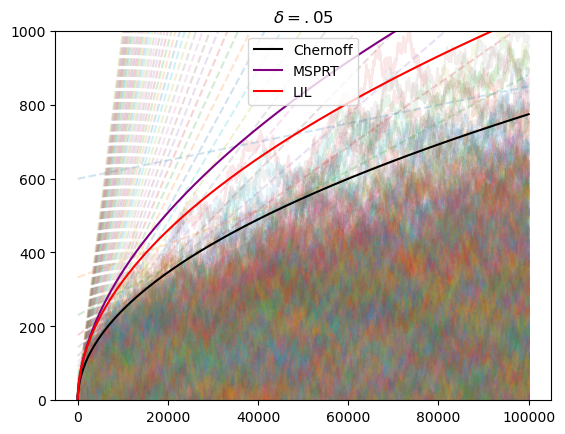
\includegraphics{boundaries.png}
    \caption{Chernoff, MSPRT, and LIL boundaries. Note that the Chernoff boundary is the pointwise minimum at each time of the set of linear boundaries. }
    \label{fig:boundaries}
\end{figure}


The previous example established a linear boundary that is always-valid. As we discusses, the fixed-time Chernoff-bound we saw above is the minimum of these linear bounds at each time $t$ - but unfortunately, it doesn't form an always-valid confidence interval.

If we are testing a null-hypothesis versus an alternative, and we suspect that the alternative is at $\Delta$, then we would use the linear boundary $\ell(\Delta, \delta)$. If instead, we believed it was in a set of fixed effects $\Delta_1, \cdots, \Delta_n$, we could consider using multiple lines to define a boundary. More general, we may take a prior distribution over the various lines. The MSPRT makes this concrete.


Let $p(\lambda)$ be a distribution over $\lambda$ and define \[M_t = \int M_t(\lambda) dp(\lambda).\]
Then $\{M_t\}_{t=0}^{\infty}$ defines a super-martingale.
\begin{align*}
    \E[M_t|\mc{F}_{t-1}] 
    &= \E\left[\int M_t(\lambda)dp(\lambda)|\mc{F}_{t-1}\right] \\
    &= \int \E[M_t(\lambda)|\mc{F}_{t-1}] dp(\lambda) \\
    &\leq \int M_{t-1}(\lambda) dp(\lambda) \\    
    &= M_{t-1}.
\end{align*}

A reasonable choice of $h(\lambda) = \frac{1}{\sqrt{2\pi \rho^2}} e^{-\lambda^2/2\rho^2}$. Then
\begin{align*}
    M_t
    &= \frac{1}{\sqrt{2\pi \rho^2}} \int e^{\lambda S_t - \frac{t\lambda^2}{2} - \frac{\lambda^2}{2\rho^2} } d\lambda \\
    &= \frac{1}{\sqrt{2\pi \rho^2}} \int e^{\lambda S_t - \frac{\lambda^2}{2}(t+1/\rho^{2})} d\lambda\\
    &= \frac{1}{\sqrt{2\pi \rho^2}} \int e^{\frac{S_t^2}{2(t+\rho^{-2})} - \frac{(S_t(t+\rho^{-2})^{-1}-\lambda)^2}{2(t+\rho^{-2})}} d\lambda \\
    &= \frac{1}{\sqrt{2\pi \rho^2}} \int e^{\frac{S_t^2}{2(t+\rho^{-2})} - \frac{(S_t(t+\rho^{-2})^{-1}-\lambda)^2(t+\rho^{-2})}{2}} d\lambda \\
    &= \frac{\sqrt{(t+\rho^{-2})^{-1}}}{\sqrt{2\pi (t+\rho^{-2})^{-1} \rho^2}} e^{\frac{S_t^2}{2(t+\rho^{-2})}}\int e^{- \frac{(S_t(t+\rho^{-2})^{-1}-\lambda)^2(t+\rho^{-2})}{2}} d\lambda \\
    &= \sqrt{\frac{\rho^{-2}}{t+\rho^{-2}}} e^{\frac{S_t^2}{2(t+\rho^{-2})}}
\end{align*}

Now by Ville's Inequality, 
\[\P(\exists t, \log(M_t) > \log(1/\delta) )\leq \delta\]
which is equivalent to the statement that with probability greater than $1-\delta$
\[|S_t| \leq \sqrt{\frac{t + \rho^{-2}}{\rho^{-2}}\log\left(\frac{t+\rho^{-2}}{\rho^{-2} \delta^2}\right)}\]
Taking $\rho = 1$ we see that 
\[\P\left(\exits t: |S_t| \geq \sqrt{(t+1)\log\left(\frac{t+1}{\delta^2}\right)}\right) \leq \delta\]

\begin{figure}
    \centering
    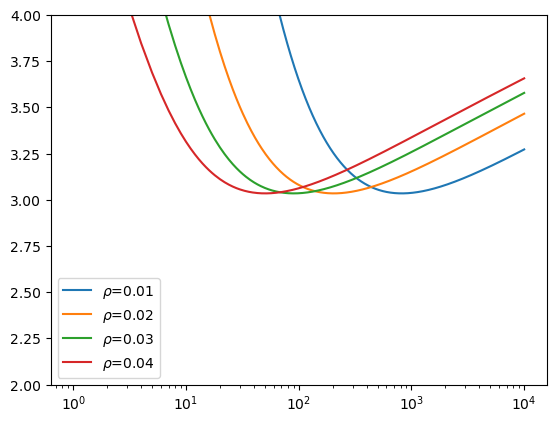
\includegraphics[width=.5\linewidth]{sprt.png}
    \caption{$u(t)/\sqrt{t}$ for various values of $\rho$}
    \label{fig:my_label}
\end{figure}

How do we choose $\rho$ ? Essentially the idea is given by Figure \ref{fig:}. Setting $u(t) = \sqrt{\frac{t + \rho^{-2}}{\rho^{-2}}\log\left(\frac{t+\rho^{-2}}{\rho^{-2} \delta^2}\right)}$, we have plotted $u(t)/\sqrt{t}$. Effectively, considering the normalized process $S_t/\sqrt{t}$, we want to choose $\rho$ so that the resulting boundary $u(t)/\sqrt{t}$ is minimized at an appropriate time $t_0$. In practice, this means that if you have the budget for a two week experiment, choose set $t_0$ appropriately and then solve for the value of $\rho$ which results in a curve pinching at $t_0$. See \cite{howard2021time} for more details. 


\noindent\textbf{Law of Iterated Logarithm.}

A natural question to ask is how to choose the tightest possible anytime confidence interval. As the discussion on the SPRT (and the MSPRT above) demonstrates, this question is not necessarily that meaningful - in practice we want to choose anytime intervals that are tight when we need them to be. A bound may be tight at a period of two weeks, but then be extremely loose after.  

Nevertheless, it's still reasonable to ask for the tightest possible anytime confidence interval \textit{asymptotically}. The answer to this is given by the law of the iterated logarithm.

\begin{theorem}
    Let $X_1, X_2, \cdots, $ be i.i.d. mean zero 1-subGaussian random variables. Then \[\lim\sup_{t\rightarrow \infty} \frac{S_t}{\sqrt{2t\log\log t}} = 1\] almost surely.
\end{theorem}

In general the LIL does not hold in finite time with a constant of 2. However, several works have provided finite time versions with slightly worse constants. The best one that I know of is from \cite{howard2021time} which shows,
\[\P(\exists t\leq 10^20: S_t\geq 1.7\sqrt{t(\log\log(e t) + 3.46)})\leq 0.025\]


\noindent \textbf{Anytime Inference in Linear Regression.} 

Imagine that we have collected a dataset $(x_1, y_1), \cdots, (x_n, y_n) \subset \mb{R}^d \times \mb{R}$ where $y_s = x_s^{\top}\theta + \epsilon_s$ where we assume $\epsilon_s$ is mean-zero $1$-sub-Gaussian noise. We also assume that $\{x_s\}_{s=1}^t$ form a \textit{fixed-design}, that is, we are assuming that the choice of $x_s$ is independent of the choice of $(x_1, y_1), \cdots, (x_{s-1}, y_s)$. 

For a minute we pretend that $\epsilon_s$ is exactly Gaussian noise with variance 1, and we assume that $V = \sum_{s=1}^t x_s x_s$ is invertible. Then recall the least-squares estimator,
\[\hat\theta_{\lambda} = \arg\min_{\theta' \in \mathbb{R}^d} \|Y - X\theta'\|^2_2, \hat{theta} = V^{-1} X^{\top} y\]
where $X = [x_1, \cdots, x_n]^{\top} \in \mathbb{R}^{n\times d}$ and $Y = [y_1, \cdots, y_n]\in\mathbb{R}^n$. 

We have that 
\begin{align*}
    \hat{\theta}
    &= V^{-1} X^{\top} y\\
    &= V^{-1} X^{\top} ( X\theta + \epsilon)\\
    &= \theta + V^{-1} X^{\top}\epsilon\\
    &= \theta + N(0, V^{-1})
\end{align*}

Thus $V^{1/2}(\hat{\theta} - \theta) \sim N(0, I)$ so that $\|\hat{\theta} - \theta\|_{V} \sim \chi^2_d$. We can now appeal to the Cramer-Chernoff method, note that for a $\chi^2_d$ random-variable, 
\begin{align*}
    
\end{align*}

We now relax the assumption that the sequence of observations is fixed in advance, and instead introduce the following assumptions
\begin{itemize}
    \item 
\end{itemize}

Now let's try this again. As above, let the least squares estimator by 
\begin{align*}
\hat{\theta} 
&= (V + \gamma I)^{-1} X^{\top}y  \\
&= (V + \lambd I)^{-1} V\theta +  (V + \lambda I)^{-1} \sum_{s=1}^t x_s\epsilon\\
&= (V + \lambda I)^{-1} V\theta +  (V + \lambda I)^{-1}M_t
\end{align*}

Now at the same time
\begin{align*}
\|\hat{\theta} - \theta\|_{V_t + \gamma I}
&= \|(V + \gamma I)^{-1} V\theta +  (V + \gamma I)^{-1}M_t - \theta\|_{V_t + \gamma I}\\
&= \|\gamma (V + \gamma I)^{-1} \theta +  (V + \gamma I)^{-1}S_t \|_{V_t + \gamma I}\\
&= \|\gamma \theta +  S_t \|_{(V_t + \gamma I)^{-1}}\\
&\leq \gamma\|\theta\|_{(V_t + \gamma I)^{-1}} + \|S_t\|_{(V_t + \gamma I)^{-1}}\\
&\leq \sqrt{\gamma}\|\theta\|_{2} + \|S_t\|_{(V_t + \gamma I)^{-1}}
\end{align*}

So the main game in town is $S_t$ - looking at it, if we could indeed conclude that the $x_s$'s were independent, standard concentration bounds would kick-in and we could easily bound it as above. However, we are allowing our sequences of $x_s$'s to be adaptive so we need a much more careful analysis. We will employ the ideas we used for the MSPRT.

To proceed, firstly note that for any $\psi\in \mathbb{R}^d$ that $M_t(\lambda) = \exp\left( \langle \lambda, S_t\rangle - \frac{\|\lambda\|_{V_t}^2}{2} \right)$ , 
where $V_t = \sum_{s=1}^t x_s x_s^{\top}$, is a super-Martingale. Then Ville's inequality automatically implies a linear boundary in this case, guaranteeing that $\P(\sup_{t\geq }\log(\bar{M}_t) \geq \log(1/\delta)) \leq \delta$

\exercise Check that $M_t$ forms a martingale sequence. 

Now, place a distribution $N(0, \gamma^{-1}I)$ over our choice of $\lambda$, and as we did with the MSPRT, we will now consider the Martingale $\bar{M}_t = \frac{1}{\sqrt{2\pi\gamma^{-d}}}\int M_t(\lambda) e^{-\frac{\|\lambda\|^2}{2\gamma^{-1}}} d\lambda$. We compute,
\begin{align*}
    \bar{M}_t 
    &= \frac{1}{\sqrt{2\pi\gamma^{-d}}}\int  e^{\langle\lambda, S_t\rangle -\frac{\|\lambda\|_{V + \gamma I}^2}{2}-\frac{\|\lambda\|^2\gamma}{2}} d\lambda\\
    &= \frac{1}{\sqrt{2\pi\gamma^{-d}}}\int e^{\frac{1}{2}\|S_t\|^2_(V_t + \gamma I)^{-1} - \frac{1}{2}\|(V_t + \gamma I)^{-1} S_t - \lambda\|^2_{V_t + \gamma I}} d\lambda\\
    &= \frac{|V_t + \gamma I|^{-1/2}}{\gamma^{-d/2}}\int e^{\frac{1}{2}\|S_t\|^2_(V_t +\gamma I )^{-1}} 
\end{align*}

Plugging this into our confidence inequality above, gives that with probability greater than $1-\delta$, for all $t\geq 0$
\[\|S_t\|_{V_t(\lambda)^{-1}} \leq \sqrt{2\log(1/\delta) + \log{\frac{|V_t + \gamma I|}{\gamma^d}}}\]

It remains to bound the second term under the square root. 



Firstly, we state the punch-line.






\bibliographystyle{alpha}
\bibliography{sample}

\end{document}I